\documentclass{beamer}

\usepackage{beamerthemesplit}
\usepackage{amsmath}
\usepackage{amsfonts}
\usepackage{amssymb}
\usepackage{qtree}
\usepackage{cancel}
\usepackage{tkz-graph}
%\usepackage[pdftex]{graphicx}

\mode<presentation>
{
  \usetheme{Warsaw}
  % or ...

  %\setbeamercovered{transparent}
  % or whatever (possibly just delete it)
}


\usepackage[english]{babel}
% or whatever

\usepackage[latin1]{inputenc}
% or whatever

\usepackage{times}
\usepackage[T1]{fontenc}

\title{Probabilistic Logical Networks}

\subtitle{Spatio-Temporal  Inference}

\author{Nil Geisweiller}

\institute[Xiamen University] % (optional, but mostly needed)
{
  Novamente LLC
}

\date[Xiamen University AGI Summer School 2009] % (optional, should be abbreviation of conference name)
{Xiamen University\\ AGI Summer School 2009}


\AtBeginSection[]
{
  \begin{frame}<beamer>{Outline}
    \tableofcontents[currentsection,currentsection]
  \end{frame}
}

\AtBeginSubsection[]
{
  \begin{frame}<beamer>{Outline}
    \tableofcontents[currentsection,currentsubsection]
  \end{frame}
}

%\newcommand{\AND}{\textit{AND}}
%\newcommand{\OR}{\textit{OR}}
%\newcommand{\NOT}{\textit{NOT}}
\newcommand{\AND}{\land}
\newcommand{\OR}{\lor}
\newcommand{\NOT}{\lnot}


\begin{document}

\frame
{
  \maketitle
}
\section[Outline]{}
\frame{\tableofcontents}

\section{Introduction}

\frame
{
  \frametitle{Spatio-temporal PLN inference overview}

  \begin{enumerate}
  \item<+-> \alert{Extract Spatio-temporal predicates} from the scene
%    (pre-processed or not)
    \begin{itemize}
    \item Spatial: {\tt inside(ball, box)}
    \item Temporal: {\tt atTime(11pm, ring(bell))}
    \item Spatio-temporal: {\tt atTime(11pm, near(Jill, John))}
    \end{itemize}
  \item<+-> Based on Spatio-temporal laws and background knowledge \alert{infer
    new predicates}
    \begin{itemize}
    \item {\tt inside(X,Y) AND inside(Y,Z)} $\Rightarrow$ {\tt inside(X,Z)}
%    \item<+-> atTime(t, drop(X) and near(X,ground) and empty\_btw(X,ground))\\
%      $\Rightarrow$ atTime(t+e, on(X, ground))
    \end{itemize}
  \item<+-> Laws and background knowledge are
    \alert{expressed in PLN}
    \begin{itemize}
    \item hand-coded
    \item learned based on past experience
    \item infered
    \end{itemize}
  \end{enumerate}

}

\frame
{
  \frametitle{Extract Spatio-temporal predicates}

  \begin{columns}

    \column{1.5in}

    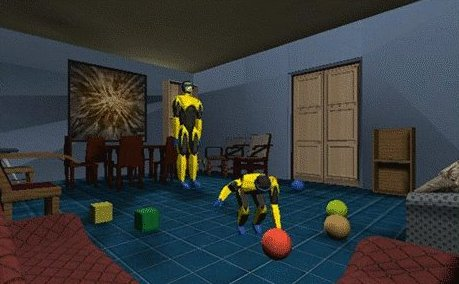
\includegraphics[scale=0.3]{agisim_crop.jpg}
    
    \column{1.5in}

    \begin{itemize}
    \item 
      {\tiny
        {\tt 
          EvaluationLink <0.99>\\
          $\ \ \ \ $near\\
          $\ \ \ \ $ListLink\\
          $\ \ \ \ \ \ \ \ $yellow\_cube\\
          $\ \ \ \ \ \ \ \ $green\_cube\\
        }
      }
    \item
      {\tiny
        {\tt 
          EvaluationLink <0.85>\\
          $\ \ \ \ $externally\_connected\\
          $\ \ \ \ $ListLink\\
          $\ \ \ \ \ \ \ \ $floor\\
          $\ \ \ \ \ \ \ \ $green\_cube\\
        }
      }
    \item
      {\tiny
        {\tt 
          EvaluationLink <0.95>\\
          $\ \ \ \ $externally\_connected\\
          $\ \ \ \ $ListLink\\
          $\ \ \ \ \ \ \ \ $floor\\
          $\ \ \ \ \ \ \ \ $yellow\_cube\\
        }
      }
    \end{itemize}

  \end{columns}
  \pause
  \begin{itemize}
  \item<+-> Can be \alert{pre-processed independently} (Computer Vision)
  \item<+-> or in tight \alert{interaction with PLN/OpenCog} (feedback to
    correct predicate extraction)
  \end{itemize}
}

\frame
{
  \frametitle{Extract Spatio-temporal predicates, \alert{OpenCog} (for now)}

  \begin{columns}
    
    \column{1.5in}

    \includegraphics[scale=0.35]<1>{filled_grid.pdf}
    \includegraphics[scale=0.35]<2>{filled_grid1.pdf}
    \includegraphics[scale=0.35]<3>{filled_grid2.pdf}
    \includegraphics[scale=0.35]<4>{filled_grid3.pdf}
    \includegraphics[scale=0.35]<5>{filled_grid4.pdf}
    \includegraphics[scale=0.35]<6>{filled_grid5.pdf}
    \includegraphics[scale=0.35]<7>{filled_grid5_near.pdf}
    
    \column{1.5in}

    \visible<7->{
    {\scriptsize
      {\tt
        \begin{tabular}{|l|}
          \hline
          AtTime\\
          $\ \ \ \ $5\\
          $\ \ \ \ $EvaluationLink\\
          $\ \ \ \ \ \ \ \ $near\\
          $\ \ \ \ \ \ \ \ $ListLink\\
          $\ \ \ \ \ \ \ \ \ \ \ \ $yellow\_obj1\\
          $\ \ \ \ \ \ \ \ \ \ \ \ $red\_obj\\
          \hline
        \end{tabular}
      }
    }
    }

  \end{columns}

  2D or 3D \alert{SpaceMap}
  \begin{itemize}
  \item<+-> \alert{Grid}, objects placed on the grid
  \item<+-> \alert{recorded} over time
  \item<7-> \alert{Fixed set of spatial predicates} (near, inside, above, etc)
    computed and \alert{timestamped}
  \end{itemize}
}

\frame
{
  \frametitle{Spatio-temporal Inference}

  Spatio-temporal PLN inference is not much different than
  other kind of PLN inference.\\[2ex]

  \pause

  \begin{beamerboxesrounded}{\alert{In practice}}
    \begin{itemize}
    \item \alert{hand-coded} Spatio-temporal inference
      rules in PLN (ImplicationLink)
    \item \alert{Dedicated} inference control mechanism
    \end{itemize}
  \end{beamerboxesrounded}
}

\section{Spatial Inference}

\frame
{
  \frametitle{Spatial inference: Region Connection Calculus}

  \begin{enumerate}
  \item<+-> Predefined set of topological spatial relationships
    
    \begin{center}
      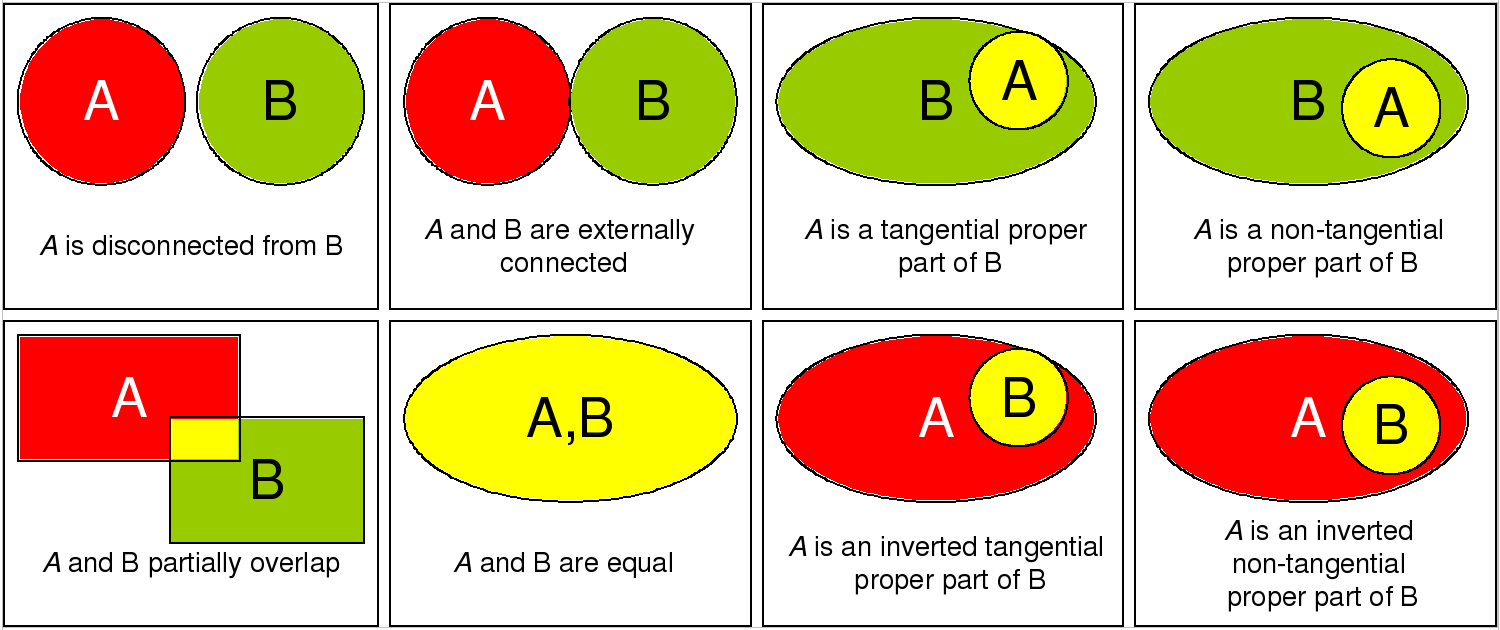
\includegraphics[scale=0.2]{RCC.png}
    \end{center}
    
  \item<+-> Rules to infer new relationships

    \visible<2>{
    \only<1,2>{
      \begin{columns}
        
        \column{1in}
        
        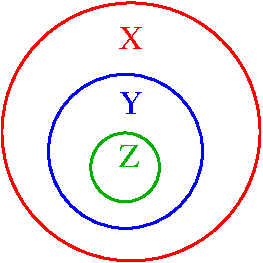
\includegraphics[scale=0.4]{NTP.pdf}
        
        \column{2in}
        
        {\tiny
          {\tt 
            ImplicationLink\\
            $\ \ \ \ $AND\\
            $\ \ \ \ \ \ \ \ $nonTangentialProperPart(\$X,\$Y)\\
            $\ \ \ \ \ \ \ \ $nonTangentialProperPart(\$Y,\$Z)\\
            $\ \ \ \ $nonTangentialProperPart(\$X,\$Z)\\
          }
        }
        
      \end{columns}
    }
    }
    \only<3>{
      \begin{columns}
        
        \column{1in}
        
        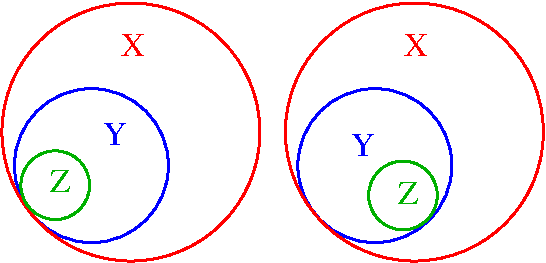
\includegraphics[scale=0.4]{TP.pdf}
        
        \column{2in}
        
        {\tiny
          {\tt 
            ImplicationLink\\
            $\ \ \ \ $AND\\
            $\ \ \ \ \ \ \ \ $tangentialProperPart(\$X,\$Y)\\
            $\ \ \ \ \ \ \ \ $tangentialProperPart(\$Y,\$Z)\\
            $\ \ \ \ $XOR\\
            $\ \ \ \ \ \ \ \ $tangentialProperPart(\$X,\$Z)\\
            $\ \ \ \ \ \ \ \ $nonTangentialProperPart(\$X,\$Z)\\
          }
        }
        
      \end{columns}
    }
    
  \end{enumerate}
  
%tangentialProperPart(A,B) ^ tangentialProperPart(B,C) 
% tangentialProperPart(A,C)  nonTangentialProperPart(A,C)

}

\frame
{
  \frametitle{Spatial inference: extending Region Connection Calculus}

  \begin{enumerate}
  \item<+-> Adding \alert{more topological predicates}
    \begin{itemize}
    \item {\tt convex} 
\includegraphics[scale=0.3]{convex.pdf}
    \item {\tt inside} 
\includegraphics[scale=0.3]{inside.pdf}
    \item {\tt partly\_inside} 
\includegraphics[scale=0.3]{partly_inside.pdf}
    \item {\tt outside} 
\includegraphics[scale=0.3]{outside.pdf}
    \item $\ldots$
    \end{itemize}
  \item<+-> Adding \alert{metrical predicates}
    \begin{itemize}
    \item {\tt near} 
\includegraphics[scale=0.4]{near.pdf}
    \item {\tt next} 
\includegraphics[scale=0.4]{next.pdf}
    \item $\ldots$
    \end{itemize}
%  \item<+-> If object have orientation, {\tt in\_front\_of},
%    {\tt to\_the\_left\_of}, $\ldots$
  \item<+-> \alert{Probabilistic or Fuzzy extension} (natural in PLN)
  \end{enumerate}
}

\section{Temporal Inference}

\frame
{
  \frametitle{Temporal Inference: Allen's Interval Algebra}

  \begin{enumerate}

  \item<+-> Predefined set of topological temporal relationships
    \begin{center}
      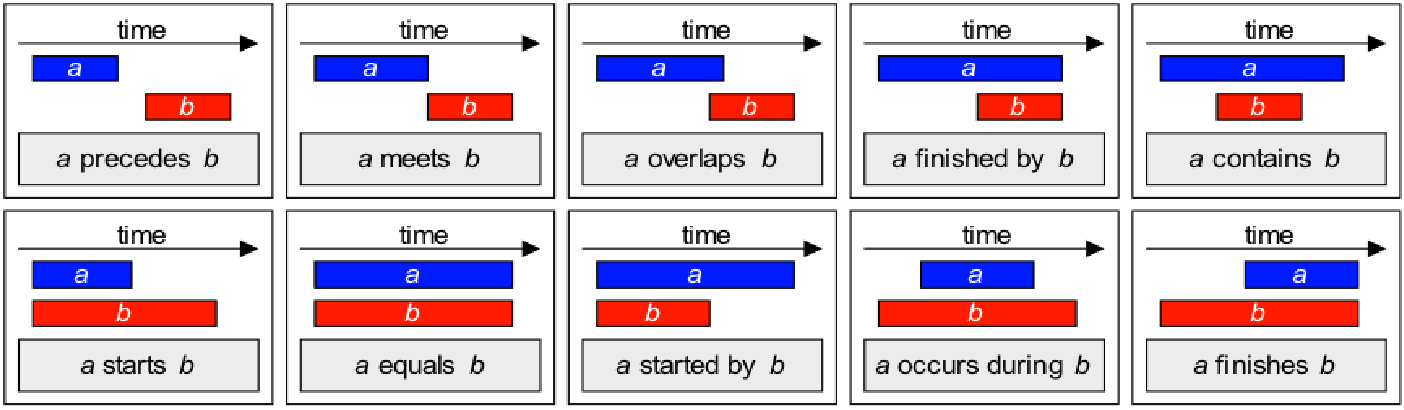
\includegraphics[scale=0.21]{Allen_trunk.png}
    \end{center}

  \item<+-> Rules to infer new relationships
    \visible<2>{
      \only<1,2>{
        \begin{columns}
          
          \column{1in}
          
          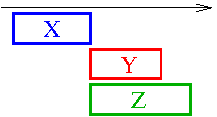
\includegraphics[scale=0.5]{mett_start.pdf}
          
          \column{2in}
          
          {\tiny
            {\tt 
              ImplicationLink\\
              $\ \ \ \ $AND\\
              $\ \ \ \ \ \ \ \ $meet(\$X,\$Y)\\
              $\ \ \ \ \ \ \ \ $start(\$Y,\$Z)\\
              $\ \ \ \ $meet(\$X,\$Z)\\
            }
          }
          
        \end{columns}
      }
    }
    \only<3>{
      \begin{columns}
        
        \column{1in}
        
        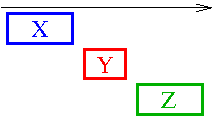
\includegraphics[scale=0.5]{precedes.pdf}
        
        \column{2in}
        
        {\tiny
          {\tt 
            ImplicationLink\\
            $\ \ \ \ $AND\\
            $\ \ \ \ \ \ \ \ $precede(\$X,\$Y)\\
            $\ \ \ \ \ \ \ \ $precede(\$Y,\$Z)\\
            $\ \ \ \ $precede(\$X,\$Z)\\
          }
        }
        
      \end{columns}
    }
    
  \end{enumerate}

}

\frame
{
  \frametitle{Spatial inference: extending Allen's Interval Algebra}

  \begin{enumerate}
  \item<+-> Quantitatif time\\
    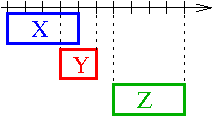
\includegraphics[scale=0.8]{quant_time.pdf}\\
    {\tiny
    {\tt initiatedAt(0,{\color{blue}\$X}),
      terminatedAt(5,{\color{blue}\$X})},\\
    {\tt initatedAt(4,{\color{red}\$Y}),
      terminatedAt(6,{\color{red}\$Y})},\\
    {\tt initatedAt(7,{\color{green}\$Z}),
      terminatedAt(11,{\color{green}\$Z})}\\
    }
%   \item<+-> Quantifiers over time\\
%     {\tiny
%       {\tt
%         Exists \$T, \$X, \$Y\\
%         $\ \ \ \ $ImplicationLink\\
%         $\ \ \ \ \ \ \ \ $initiatedAt(\$T,\$X)\\
%         $\ \ \ \ \ \ \ \ $initiatedAt(\$T+3,\$Y)\\
%       }
%     }
  \item<+-> Probabilistic and Fuzzy extension\\
  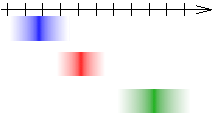
\includegraphics[scale=0.8]{fuzzy_quant_time.pdf}
  \item<+-> Temporal logic, etc
  \end{enumerate}
}

%\section{Example of Spatio-temporal Inference}

\frame
{
  \frametitle{Example of Spatio-temporal Inference}

  Assessing the
  \alert{probability of being in the airport an hour before my flight}
  considering I set my \alert{alarm clock at 5am}.
  \pause
  \begin{beamerboxesrounded}{Axioms}
    {\tiny
    {\tt
    \begin{enumerate}
    \item<+-> atTime(5am, alarm\_clock) <1>
    \item<+-> ForAll \$T\\
      $\ \ \ \ $ImplicationLink <0.9>\\
      $\ \ \ \ \ \ \ \ $atTime(\$T, alarm\_clock)\\
      $\ \ \ \ \ \ \ \ $atTime(\$T+5mn, waking\_up)\\
    \item<+-> ForAll \$T\\
      $\ \ \ \ $ImplicationLink <0.9>\\
      $\ \ \ \ \ \ \ \ $atTime(\$T, waking\_up)\\
      $\ \ \ \ \ \ \ \ $atTime(\$T+25mn, grab\_a\_cab)\\
    \item<+-> ForAll \$T\\
      $\ \ \ \ $ImplicationLink <0.8>\\
      $\ \ \ \ \ \ \ \ $atTime(\$T, grab\_a\_cab)\\
      $\ \ \ \ \ \ \ \ $atTime(\$T+30mn, inside(self, airport\_parking))\\
%     \item<+-> ForAll \$T1\\
%       $\ \ \ \ $ImplicationLink <0.9>\\
%       $\ \ \ \ \ \ \ \ $initiatedAt(\$T1, inside(self, airport))\\
%       $\ \ \ \ \ \ \ \ $AND
%       $\ \ \ \ \ \ \ \ \ \ \ \$\$T2>\$T1+1h\\
%       $\ \ \ \ \ \ \ \ \ \ \ \$terminatedAt(\$T2, inside(self, airport))\\
    \item<+-> ForAll \$T\\
      $\ \ \ \ $atTime(\$T, inside(airport\_parking, airport)) <1>\\
    \item<+-> atTime(7am, flight) <1>
    \end{enumerate}
    }
    }
  \end{beamerboxesrounded}

}

\frame
{
  \frametitle{Example of Spatio-temporal Inference}
  
  \begin{beamerboxesrounded}{Spatio-temporal rule}
    {\tiny
    \begin{enumerate}
    \item<+-> At T, if X is inside Y and Y is inside Z
      then X is inside Z\\
      {\tt
      ForAll \$T, \$X, \$Y, \$Z\\
      $\ \ \ \ $ImplicationLink\\
      $\ \ \ \ \ \ \ \ $AND\\
      $\ \ \ \ \ \ \ \ \ \ \ \ $atTime(\$T, inside(\$X,\$Y))\\
      $\ \ \ \ \ \ \ \ \ \ \ \ $atTime(\$T, inside(\$Y,\$Z))\\
      $\ \ \ \ \ \ \ \ $atTime(\$T, inside(\$X,\$Z))\\
      }
%     \item<+-> In the absence of temporal information on P,
%       if P then P holds at any time\\
%       {\tt
%       ForAll \$T, \$P\\
      
%       $\ \ \ \ $ImplicationLink\\
%       $\ \ \ \ \ \ \ \ $\$P\\
%       $\ \ \ \ \ \ \ \ $atTime(\$T, \$P)\\
%       }
%     \item<+-> If P implies Q and P holds at T then Q holds at T\\
%       {\tt
%       ForAll \$T, \$P, \$Q\\
%       $\ \ \ \ $ImplicationLink <1>\\
%       $\ \ \ \ \ \ \ \ $AND\\
%       $\ \ \ \ \ \ \ \ \ \ \ \ $atTime(\$T, \$P)\\
%       $\ \ \ \ \ \ \ \ \ \ \ \ $ImplicationLink\\
%       $\ \ \ \ \ \ \ \ \ \ \ \ \ \ \ \ $P\\
%       $\ \ \ \ \ \ \ \ \ \ \ \ \ \ \ \ $Q\\
%       $\ \ \ \ \ \ \ \ \ \ \ \ $atTime(\$T, \$Q)\\
%       }
%     \item<+-> If P holds at time T and Q holds at time T, then P and Q holds
%       at time T\\
%       {\tt
%       ForAll \$T, \$P, \$Q\\
%       $\ \ \ \ $ImplicationLink <1>\\
%       $\ \ \ \ \ \ \ \ $AND\\
%       $\ \ \ \ \ \ \ \ \ \ \ \ $atTime(\$T, \$P)\\
%       $\ \ \ \ \ \ \ \ \ \ \ \ $atTime(\$T, \$Q)\\
%       $\ \ \ \ \ \ \ \ $atTime(\$T, P AND Q)\\      
%       }
    \end{enumerate}
    }
  \end{beamerboxesrounded}
}

\frame
{
  \frametitle{Example of Spatio-temporal Inference}

  \begin{beamerboxesrounded}{Target theorem}
    {\tt atTime(6am, inside(self, airport)) <?>}
  \end{beamerboxesrounded}
  
  \pause

  \begin{beamerboxesrounded}{Sub-target theorem}
    {\tt atTime(6am, inside(self, airport\_parking)) <?>}
  \end{beamerboxesrounded}
}

\frame
{
  \frametitle{Example of Spatio-temporal Inference}

  \begin{beamerboxesrounded}{Inference Steps for the \alert{sub-target theorem}\\
      {\scriptsize
        {\tt atTime(6am, inside(self, airport\_parking))
          <\only<1-6>{?}\only<7>{\alert{0.73}}>}}
    }
  {\tiny
  \begin{enumerate}
  \item<+-> Instantiate axiom 2 with {\tt \$T=5am}\\
    {\tiny
    {\tt
    ImplicationLink <0.9>\\
    $\ \ \ \ $atTime(5am, alarm\_clock)\\
    $\ \ \ \ $atTime(5:05am, waking\_up)\\
    }
    }
  \item<+-> Apply axiom 1 as premise of previous inference step\\
    {\tiny
    {\tt
    atTime(5:05am, waking\_up) <0.9>\\
    }
    }
  \item<+-> Instantiate axiom 3 with {\tt \$T=5:05am}\\
    {\tiny
    {\tt
    ImplicationLink <0.9>\\
    $\ \ \ \ $atTime(5:05am, waking\_up)\\
    $\ \ \ \ $atTime(5:30am, grab\_a\_cab)\\
    }
    }
  \item<+-> Apply the result of step 2 as premise of the previous step\\
    {\tiny
    {\tt
    atTime(5:30am, grab\_a\_cab) <0.81>
    }
    }
  \item<+-> Instantiate axiom 4 with {\tt \$T=5:30am}\\
    {\tiny
    {\tt
    ImplicationLink <0.8>\\
    $\ \ \ \ $atTime(5:30am, grab\_a\_cab)\\
    $\ \ \ \ $atTime(6am, inside(self, airport\_parking))\\
    }
    }
  \item<+-> Apply the result of step 4 as premise of the previous step\\
    {\tiny
    {\tt
      \alert<7>{atTime(6am, inside(self, airport\_parking)) <0.73>}\\
    }
    }
  \end{enumerate}
  }
  \end{beamerboxesrounded}
}


\frame
{
  \frametitle{Example of Spatio-temporal Inference}

  \begin{beamerboxesrounded}{Inference steps for the \alert{target theorem}\\
    {\scriptsize
    {\tt
    atTime(6am, inside(self, airport))
    <\only<1-4>{?}\only<5>{\alert{0.73}}>
    }
    }
  }
  {\tiny
  \begin{enumerate}
  \item<+-> Instantiate axiom 5 with {\tt \$T=6am}\\
    {\tt
    atTime(6am, inside(airport\_parking, airport)) <1>
    }
  \item<+-> Apply sub-target theorem and previous step (standard probability
    theory)\\
    {\tt
    AND <0.73>\\
    $\ \ \ \ $atTime(6am, inside(self,airport\_parking))\\
    $\ \ \ \ $atTime(6am, inside(airport\_parking,airport))\\
    }
  \item<+-> Instantiate spatio-temporal rule 1, with {\tt \$T=6am},
    {\tt \$X=self}, {\tt \$Y=airport\_parking} and
    {\tt \$Z=parking}\\
    {\tt
    ImplicationLink <1>\\
    $\ \ \ \ $AND\\
    $\ \ \ \ \ \ \ \ $atTime(6am, inside(self,airport\_parking))\\
    $\ \ \ \ \ \ \ \ $atTime(6am, inside(airport\_parking,airport))\\
    $\ \ \ \ $atTime(6am, inside(self,airport))\\
    }
  \item<+-> Apply step 2 as premise of previous step\\
    {\tt
      \alert<5>{atTime(6am, inside(self, airport)) <0.73>}
    }
  \end{enumerate}
  }
  \end{beamerboxesrounded}
}

% \frame
% {
%   \frametitle{Example of Spatio-temporal Inference}

%   \begin{beamerboxesrounded}{Target theorem}
%     {\tt atTime(6am, inside(self, airport)) <0.73>}
%   \end{beamerboxesrounded}
% }

\section{Conclusion}

\frame
{
  \frametitle{Conclusion}
  \begin{itemize}
  \item Coding Spatio-temporal laws in the atomSpace
  \item Getting spatio-temporal knowledge (computer vision)
  \item In practice, \alert{inference control} will play
    a great role to lead to efficient inference
  \end{itemize}
}

\end{document}
